\documentclass[12pt, a4paper]{article}
\usepackage{minted}
\usepackage{multirow}
\usepackage{enumerate}
\usepackage{geometry}
%\geometry{left=5cm,right=5cm,top=2.5cm,bottom=2.5cm}
\usepackage{fontspec}
\setmainfont{Times New Roman}
\usepackage{minted}
\usepackage[slantfont,boldfont]{xeCJK}
\setCJKmainfont{SimSun}
%% \usepackage{indentfirst}
%% \setlength{\parindent}{2em}
\usepackage{float}
\usepackage{titling}
\usepackage{graphicx}
\usepackage{subfigure}
\usepackage[square,sort,comma,numbers]{natbib}
\usepackage{booktabs}
\usepackage{amsmath}
\usepackage{titlesec}
\usepackage{url}
\setCJKmonofont{SimHei}
\input zhwinfonts
\setlength{\bibsep}{0.5ex}

\titleformat{\section}{\normalsize\bfseries}{}{0em}{}
\titlespacing{\section}{0pt}{1em}{0em}

\pretitle{\begin{center}\LARGE}
\posttitle{\par\end{center}\vskip 0.5em}
\preauthor{\vspace{8cm}\begin{center}
    \large \lineskip0.5em %
    \begin{tabular}[t]{c}}
\postauthor{\end{tabular}\par\end{center}}
\predate{\begin{center}\large}
\postdate{\par\end{center}}
\renewcommand\figurename{图}

\begin{document}

\title{{\bf\Huge Analysis of Different Implementations of Bitmap Index}}
\author{\emph{Harbin Institute of Technology}\\\emph{Department of Computer Science and Technology}\\Ma Yukun\\1150310618}

\date{2017/11/18}

\nocite{*}

%% \maketitle\setcounter{page}{0}\thispagestyle{empty}
%% \newpage
%% \tableofcontents

\begin{figure}[H]
  \centering
  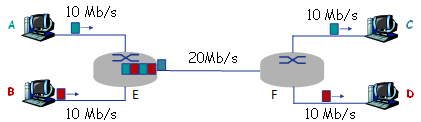
\includegraphics[width=4in]{figures/img.png}
  \caption{题图}\label{fig:img}
\end{figure}

如图\ref{fig:img}所示,设左侧的中间节点为E,右侧的中间节点为F。

设从A发送的$2Mbits$文件为文件1,从B发送的$1Mbits$文件为文件2

\section{(1)}

在使用报文交换时,对于A发送的$2Mbits$的文件1来说:

文件1完全发送到E时的时间为$$t_{E1}=\frac{2}{10}=0.2s$$

文件1完全发送到F时的时间为$$t_{F1}=t_{E1}+\frac{2}{20}=0.3s$$

文件1完全发送到C时的时间为$$t_{C}=t_{F1}+\frac{2}{10}=0.5s$$

因此文件1从A发送到C所需时间为$$t_{1}=t_{C}=0.5s$$


对于B发送的$1Mbits$的文件2来说:

文件2完全发送到E时的时间为$$t_{E2}=0.1+e+\frac{2}{10}=0.3+e (s)$$

由于文件1需要由E发送到F,文件B所需要的等待时间为$$t_w=t_{E2}-(t_{F2}) = e (s)$$

文件2完全发送到F时的时间为$$t_{F2}=t_{E2}+t_w+\frac{1}{20}=0.35 +e (s)$$

文件2完全发送到D时的时间为$$t_{D}=t_{F2}+\frac{1}{10}=0.45+e (s)$$

故文件2从B发送到D所需时间为$$t_{2}=t_{D}-(0.1+e)=0.45+e-(0.1+e)=0.35 (s)$$

\section{(2)}

文件1最后一个分组发送到E时的时间为$$t_{E1}=\frac{2}{10}=0.2s$$

因为$20>=10+10$,E到F的链路未发生阻塞,故文件1最后一个分组从E发送到F的速率为$20Mbps$,因此文件1最后一个分组到达F的时间为$$t_{F1}=t_{E1}+\frac{1kbits}{20Mbps}=0.20005s$$

文件1最后一个分组发送到C时的时间为$$t_{C}=t_{F1}+\frac{1kbits}{10Mbps}=0.20005+\frac{1}{10000}=0.20015$$

故文件1从A发送到C所需时间为$$t_1=t_C=0.20015s$$

文件2最后一个分组发送到E时的时间为$$t_{E2}=0.1+e+\frac{1}{10}=0.2+e (s)$$

同上,文件2最后一个分组发送到F时的时间为$$t_{F2}=t_{E2}+\frac{1kbits}{20Mbps}=0.20005+e(s)$$

文件2最后一个分组到达D时的时间为$$t_{D}=t_{F2}+\frac{1kbits}{10Mbps}=0.20015+e(s)$$

故文件2从B发送到D所需时间为$$t_2=t_D-(0.1+e)=0.20015+e - (0.1+e) = 0.10015 s$$


\section{(3)}

如果将用时看做数据量的函数,那么对于报文交换来说,由从A发送2Mbits文件到C需要0.5s,该文件的传输速率为:

$$v_1=\frac{2Mbits}{0.5s}=4Mbps$$

从B发送1Mbits文件到D需要0.35s,该文件的传输速率为:

$$v_2=\frac{1Mbits}{0.35s}\approx 2.857Mbps$$

两者的速度比例$$k_1=\frac{v_1}{v_2}\approx 1.4$$

而对于分组交换来说,由从A发送2Mbits文件到C需要0.5s,该文件的传输速率为:

$$v_1=\frac{2Mbits}{0.20015s}\approx 9.993Mbps$$

从B发送1Mbits文件到D需要0.35s,该文件的传输速率为:

$$v_2=\frac{1Mbits}{0.10015s}\approx 9.985Mbps$$

两者速度比例$$k_2=\frac{v_1}{v_2}\approx 1.0$$

从速度比例来看,使用报文交换时,两个文件的传输速率差别较大,公平性较差。而在使用分组交换时,传输速率差别较小,速度比例接近1,更为{\textbf 公平},更加符合“传输数据量小用时少,传输数据量大用时长”的要求。

%% \renewcommand\refname{Reference}
\end{document}
